\documentclass{article} \usepackage[utf8]{inputenc}
\usepackage{xstring}
\usepackage{calc, xintexpr}
\usepackage{xfp}
\usepackage{pdftexcmds}
\usepackage{coolstr}
\usepackage{intcalc}
\usepackage{amsrefs}
\usepackage{graphicx}
\usepackage{hyperref}
\usepackage{listings}
\usepackage[most]{tcolorbox}
\usepackage{lipsum}

% quote backgrounds: https://tex.stackexchange.com/a/436253/102826
\definecolor{linequote}{RGB}{224,215,188}
\definecolor{backquote}{RGB}{249,245,233}

\newtcolorbox{myquote}{%
    enhanced, breakable, 
    size=fbox,
    frame hidden, boxrule=0pt,
    sharp corners,
    colback=backquote,
    borderline horizontal={.5pt}{0pt}{linequote},
    borderline horizontal={.5pt}{1pt}{linequote}
}

%% Important!!
%% Use ! before "O{}" with xparse 2018-05-12 
%% See: https://tex.stackexchange.com/q/434928/1952
\NewTCBListing{mycode}{ !O{} }{%
    enhanced, breakable, 
    size=fbox,
    frame hidden, boxrule=0pt,
    sharp corners,
    colback=gray!30,
    listing only, 
    listing options={%
        style=tcblatex,
        keywordstyle=\color{brown!70!black},
        texcsstyle=*\color{brown!70!black}
    },
    #1}


% TeX docs at http://pgfplots.sourceforge.net/TeX-programming-notes.pdf

% TODO: https://tex.stackexchange.com/questions/29402/how-do-i-make-my-document-look-like-it-was-written-by-a-cthulhu-worshipping-madm
% cool hack: http://texhacks.blogspot.com/2010/12/forcing-full-expansion.html

\newif\ifcomputationenabled
\computationenabledtrue
\newif\ifdebug
\debugtrue

\title{Advent of Code\\
{\large Day Eight}}
\author{LucidBrot} \date{August 2020}
\newcommand\Strawberries{34}


% https://tex.stackexchange.com/a/7183/102826
% if is num, emphasize, else ignore.
\def\isnum#1{%
  \if!\ifnum9<1#1!\else_\fi
    \emph{#1}\else#1\fi}


\newcommand{\firstchar}[1]{%
    \StrLeft{#1}{1}[\firstletter]%
    \firstletter
}

% documentation: \getchar[hello]{5}   is 'h'
\def\getchar[#1]#2{%
\StrMid{#1}{#2}{\numexpr #2 + 0\relax}[\mychar]%
\mychar}

% same as getchar but maybe it works when used in string comparison?
\def\getcoolchar[#1]#2{%
\substr{#1}{#2}{1}%
}
% NOPE! It's just as broken, just in a different way. it works as long as the first argument is a string. but if it's a command... then it returns the whole thing as first character.

% https://tex.stackexchange.com/questions/195491/ifthenelse-equal-string-comparison-fails
\makeatletter
\newcommand\strcmptozero[1]{%
  \ifnum\pdf@strcmp{\unexpanded{#1}}{0}=0 %
     \expandafter\@firstoftwo
  \else
    \expandafter\@secondoftwo
  \fi
    {TRUE}
    {FALSE}%
}
\makeatother

% modulo computation in plain TeX
% https://tex.stackexchange.com/a/34434/102826
\newcount\tmpcnta
\def\modulo#1#2{\tmpcnta=#1
        \divide\tmpcnta by #2
        \multiply\tmpcnta by #2
        \multiply\tmpcnta by -1
        \advance\tmpcnta by #1\relax
        \the\tmpcnta}

\begin{document}


\maketitle

\section{About}
The task at \href{https://adventofcode.com/2019/day/8}{adventofcode 2019 day 8} is fairly straightforward itself. It can be summarized as \begin{myquote}\begin{quote}
Read the input line of $N$ numeric characters into \textit{layers} of size $width * height$ (which are known) to find the layer that contains the lowest number of zeros. Then return the number of \texttt{'1'} digits multiplied by the number of \texttt{'2'} digits within that layer.
\end{quote}\end{myquote}

However, we're doing this in \LaTeX , which is typeset in spongebob-case for a reason.

\section{The \LaTeX\,\.E\.x\.p\.e\.r\.i\.e\.n\.c\.e}
First of all, we're doing something that it was not meant to be used for -- so that means we never get the search results we want. Searching about arrays in \LaTeX for example gives you an explanation about how to typeset matrices. Very useful, but not what I wanted. Thankfully, the \href{http://pgfplots.sourceforge.net/TeX-programming-notes.pdf}{pgfplots sourceforge page} contains a pdf with \textit{Notes On Programming in \TeX}.

Secondly, there don't seem to be any variables. Just \textit{counters}, \textit{counts} which are the \TeX version. and \textit{ifdefs} and most importantly \textit{macros}. But I did not read up on the internals of \TeX and \LaTeX, so I have no clue about the exact way that macros are evaluated. Sometimes you can define a command that works perfectly well for a constant argument, but if you dare use it on the result of another command, you're being had from multiple directions. Because that result has not already been evaluated (expanded) and is passed as-is into the other command. My version of pdfLaTex does not feature the primitive \texttt{\textbackslash expanded} yet. Using \texttt{\textbackslash expandafter} feels very clunky. Luckily there's a hack around that to be found \href{http://texhacks.blogspot.com/2010/12/forcing-full-expansion.html}{here}. And sometimes the problem was actually the \texttt{xstring} package which also breaks the hack.

\begin{samepage}
\begin{myquote}
\begin{quote}
The macros of this package are not purely expandable, i.e. they cannot be put in the argument of an \textbackslash edef. Nestling macros is not possible neither.

For this reason, all the macros returning a result (i.e. all excepted the tests) have an optional argument in last position. The syntax is \texttt{[ name ]}, where name is the name of the control sequence that will receive the result of the macro: the assignment is made with an \textbackslash edef which make the result of the macro name purely expandable. Of course, if an optional argument is present, the macro does not display anything.\citelist{\cite{Gonzalo}}
\end{quote}
\end{myquote}
\end{samepage}

After eliminating some problems of this sort by storing the result in a new command by virtue of the optional argument, the same problem still appeared because some commands just don't work due to the same issue, even if they are making use of the optional argument to return that in turn \hbox{(See Figure \ref{code:1}, Figure \ref{fig:diff}).}

\begin{figure}[hbtp]
\begin{lstlisting}[language=TeX]
\def\getchar[#1]#2{%
\StrMid{#1}{#2}{\numexpr #2 + 0\relax}[\mychar]%
\mychar}
\end{lstlisting}
\caption{This command does not like to be used on a non-constant string.}
\label{code:1}
\end{figure}

\begin{figure}[hbt]
\makebox[\textwidth][c]{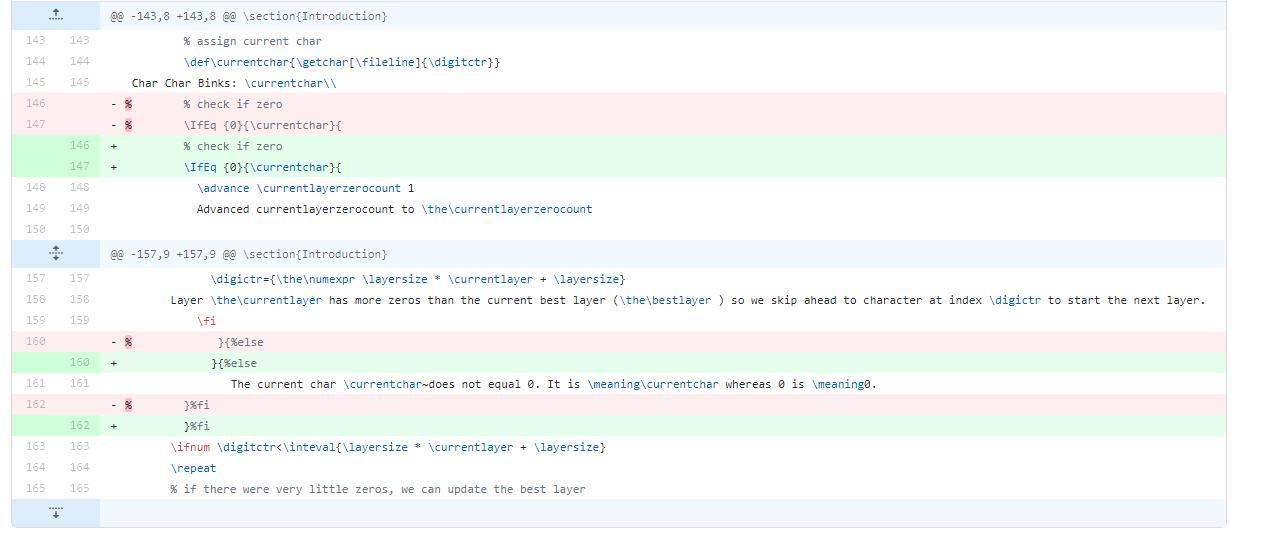
\includegraphics[width=1.6\textwidth]{diff}}%
  \caption{The difference between wrong code that compiles (red) and seemingly correct code that produces a compiler error (green).}
  \label{fig:diff}
\end{figure}

Finally, the performance of the \texttt{xstring} package is whack. It takes more than two minutes to figure out the length of a 15'000 character string. The bash command \texttt{wc -c inputfile.txt} does that in less than a second.
\clearpage
\section{Execution}

We had \Strawberries\ Strawberries for this year's harvest. Probably not enough.
So we are sad now and solve https://adventofcode.com/2019/day/8.

% get first character of string hello
\getchar[hello]{1}
\getcoolchar[hello]{2}
%\firstchar{122222222021222212220220022122202222022012222222222222022022122222220210000222222222222112222222222022222222222222222222222222022022222222222222222222022222222220222202120221122222212222122202222222222222022222222222222210010222222222222202222222222022222222222222222222222222022222222222222222222222022222222222222212021221222222212222222002222222222222022022022222221201000222222222222202222222222122222222222222222222222222122222222222222222222222122222222122222202022220222022222222122102222222222222122222222222220202202222222222222012222222222222222222222222222222222222222122222222222222222222222222222222222222122222022002212222222002222222222222122022122222221210200222222222222122222222222022222222222222222222222222022022222222222222221222022222222222122212121220222122202222122022222222222222122022222222221222212222222222222202222202222022222222222022222222222222222122222222222222222222222222222222222222121222222102222222222212222222222222222022022221221201212222222222222122202212222122222222222022222222222222122222222222222222222222122222222222222222122222222222202222022122222222222222122222022220220211010222222222222202212202222122222222222022222222222222022022222222222222220222122222222020222222020222022102202222122212222222222222222122022220211220210222222222222202222212222122222222222022222222222222222022222222222222221222122222222122122212021221122212212222022002222222222222222022022222212202020222222222222122222212202122222222222122212222222222122222222222222222222222222222222121122212020221022112202222022122222222222222022022122220202221220222222222222012202212222222222222222022222222222222222122222222222222221222222222222222122202220221022102222222222012222222222222222120122222202200210222222222222222222202212022222222222122202222222222222222222022222222220222222222222220222202020220222122222222222102222222222222122122022220210220122222222222220012212222222222222222222222222222222222222122222022222222221222022222222122222222120221222000202222222222202222222222222021122221202200011222222222222002202202212222222222222122202222222222022122222022222222220222122222222022222202020221122201202222022112212222222222022020022221201210021222222222220002202202212022222222222122202222222222122022222022222222222222022222222022222202221221022111202202222122222222222222122221122221221210200222222222222002222222212122222222222022212222222222122222222222222222220222122222222020122222122222222102212212122212202222222222122020022221201220120222222222220202222212202222222222222022212222222222222122222122222222220222022222222021022222221221022112202202122202212222222222122020122220202221010222222222221122212212222122222222222222222222222222122222222222222222221222122222222221022202222222222022222212122112222222222222022022222220210221220222222202220002222212222122222222222122222222222222022222222122222222220222222222222220222202121220022122222212122122202222222222122222222221202201022222222222221222202222222122222222222222212222222222122222222022222122222222222222222221222202121220022010222202022112222222222222122021122222211211221222222202222202222202222122222222222022222222222222122022222122222222220222122222222220220222120221222012222222222202202222222222222221022220201211222222222212220012202222212022222222222222202222222222022222222122222222221222022222222222120212022220022000202222022122212222222222022022022221222200210222222212221212202212222222222222222122212222222222022122222022222022221222122222222020022222120221022121112222122102212222222222222021022220212202011222222202220012202202212222222222222222212022222222022022222222222022222222022222222220020202121220022112022202022022222222222222222221022220210210110222222222220102202202222222222222222022212022222222122022222222222122220220022222222221021212121220022122222212222112202222222222122121222222211200210222222222221002212212202022222222222022212222220222222222222122222022221222022222222122220212221220222010222122122122202222222222222121122221212220100222222222220122202212212222222222222122222122202222021222222122222022222221022222222222021222120222122112002202122022212222222220022222222220212202222222222212220012212212222122222222222022222122220222022222222122222222220221222222222120221212221221222221212022222212222222222221222220222222201212100122222202221022202222202022222222222122222022220222120022222122222222221222022220222122220212222220222211002102222012202222222221022122122220221202122122222202222222212212222022222122222122202122211222020222222022222022221221222222222121120222022222222101002122022222212222222222222120022220212211112022222222222112212212212122222022222122222222210222121022222122222122222220122220212222121202021222212202212122222102222222222220022221122221212220211122222212221022212202212022222122222022202022200222020222222222222122221221122220222122021222120222012200112102122212212222222221122022122221220222121222222222220222222212202122222222222122202122211222222122222022222222221222022220212121220212020221202220012022222222202222222221022222022220221202102222222222222222222222212122222122222222222002211222121122222222222222221222222220222221120212220222122212202012022022222222222222122220222220200221101222022202221122202202202022222022222222212212201222120022222022222122222220222221212022021202221222002001112012122212202222222222222122122220201200122122022212221222222202202222222222222122212222200222022022222022222022220222222220212022220202121220212201202022022112222222222222122021122222221202220122122202220112212212222122222222222022202022222222120122222022222222221222022222222021121202221220122201212022122222222222222220122120022222221211001122222212222222212212202122222022222122202012220222121222222122222122220221022222202122120202120221002120202212122022202222222220122221022221221212222022022202220002212202212222222222222222222212200222122122222022222122221221022221202022221202022222112000112102222222202222222222022022222222210202212222122212220012222222212222222222222022222212222222222022222222222022220220022220212121220212022221102111222002222112202222222222222222022220221211012122222222221002202202222122222222222022202202221222222122222222222222221220022222212021122202222220002011202022222102222222222220122020022221200201010222222222222122202202202022222222222222222122221222020122222022222222221202122222212022020202121222112102112122022212222222222220022020122222211221011222222222221012222222222122222222222222202112212222022022222022222122222220022122202220122102022220012012122112022122222222222221222022022220220201211221122202222222212202212122222022222222222122200222120222222022222122222200122122202222121012122221202010212202122122202222222222222122102222220202121021022222221112202222202022222002222122212102210222121222222022222122221220222020222122022122120220212202002022222222202222222222222120102221222212210020022222222202202202222222222112222022202122211222021022222222222122220220122122212220220122220221202110122012022212212222222221222122222220212202222022122222210022202212202122222022222022212122210222022022222122222222222210022120202020021122121220222222022002122022212222222221122122002222222220111220122212202102222202222122222012222022202112201202020122222022222022221221022120202221120002121221222122002222122112202222222222022222012221202210222020122222212202202222222122222012222122202012220212222222222022222222221211222022202220122222121222002121212202222102212222222222022121122221211201100221122222211212222212212122222122222122222222201202020122222122222022220220022222202122220102121222122210202212122202202222222222122220002222210211100020122212200212212222202022222122222222212102200222021022222222222022221211022220222022000022022222112102102022022122212222222222022222222220201211222020222222222112202222202122222122222222202022211202022222222022222122221210222121202022001212222220102222222212122102212222222221222120202222200200120021122212222102212202202222222102222022212022210202220022202022222122221201220120222022220202020222102202102102122012222222222221022221102221200212100121122222202022212222212122222002222122222122220202122222222122222222222221221022212122012222021222002120102112222112222222122220122220022222202211102220222202221102212222212222222102221122222112221222021222212122222022222221121022212222221022220221102020222002222122222222122222022020012221200210110020122212221002212212212222222202221222202022212212120122212021222122221220221120212022022112222221222112212012122222222222222222122021202220200212022020222222212122202222202122222122221022222002212202120022202122222122222212120122202021201022220221102220122002022010222222122221122221112221222222020122022202210222202222212022222002222222212202211202120222102122222222221202022020212122011222121221002011102112222012212222222222122020012222200212222020022212222202212202222022222122220022202202222202120222012120222122221210022020222120211012022222002001212102022102202222122222022121122221210210121022222202222102202202202222222200220122202122200212021021122021222222220200221221202221001212020222112110002122222120222222222222022222212221222220201121022222202202222202222220222122221122212202201202220021002222222122221201122200222222220122022221222102202212022212212222002221222221122222200202012022102212200012202222212221222201221122222012221212022121002121222222220221121020212021110202121222022222102222022220212220002221222221202221222221112121112202012222212202202122222222222022212202220202022122112020222122221221021111212122211112221221002021122222122210212220022221122121102222211222121020122202212112222212222022222012221022222200201212020122022221222122221220122202202021201112121221112200012112022111222122012221122120012221222222110120122212111222202212202120222211221122202020212222221021122020222222220200020112212121121002220221102122022212222201202220122220122221222222201222222221022212002122212222202021222112221022222001200202120221112021222122221211122222202122010122020222122211002212022102202122112222222120022220221211120221202212200102222212202220222200220122202112210222122120102020222022220222221002222121011202120221022220222022122200212222002222122221212221222211101021012222201012222212202022222122220222202100220222222122122021222122220202022212202122000112022220202201222121122222212220002222122120110220200211022121122222000222212212222221222010220222222120201222022121222122222022221220221020212020202222220221212110122210222001212021212222022122211222210212010220112212210012222222220222222121222222212202202222121220222021222122222212222102212122111122221220122112202122022211202022022220122221112222211220221022112212000012210222220020222100220222000212201212121121020021222222220212121112202202121222120220112211002002222022202221222220222222211222112222010221122212022102201212221022222101221022222211212202121221012120222022221220022012202222122022122210202011222211022001222202002222122221222221101201021120002222212122200202221120222020222222101021200222220020122220222122222202122120202101201022122200112022022201222111222011122220222221110220222210001221002202201022200212210221222020221022122220200202221121101121222022220220022001102002002102022222102101202212022202202221112220022222020220211201121020012222202212221202222021222201220222121201210222020121021221222122220221120122122222201102122212122002012112122012212020222220122220221221201201222101202212202202211212222022222112220222202201212202221022002122222122221202100011112102200212020202102102212121022121202000022221122121012222002220000002011202001112211222211021222102222122110101221222020020102222222022222212120011002112021122021210222222212110222121222010122222122022202220211212020010201222010112201202222122222020220022221001210212222021211022222222222211010002212122222112121221102110012120022201202102212221122122212220020212201001120222011002221022210121222220221022220021222202220220112122222022221222010222202102010102222200212011122210221212222222002220122022110222220200212220002222202022221222202021222022221122112121221222020021002121222222222222202110202102112122020200122000112000122122212211202220222021212221200210220221010222222002202212220121222122222222100020211221021221211022222222221222112101002202222212220200122002122200222100202111222220222120020222020200121010001222201112202202200221222212221022210212212222122222022121222022222110101021102112002012022202022202002010020102202221022220122022201221210212002011212222122122201222220221120012222122012220210202021220010020222022221110212210202021220202220202112002122220121221222212012220222121102221202212101201102202011112200022222021022220221122002211221222021021110021222222220201211120112002011012122201102021022222020100212022112221020122212220021221201102022222121202220102202020121002222002110121220221222022122022222222222121211112222122220002220212002121202221120022202222022222022021221221112202212112111222010212212002201222220202220102010221102210120221101222222222221102002012012120022122120210202222212022122210222200212222121220112222220202021201212222201222211202220221122221221122212202010222020120120122222022221100220212102100001002021212002111112001120212222122012220122021012221001211210222221202220212222122202020022121220002000112102201220021101120222222221101011200022121121212020210112201002012222221212002102120121020020221000210221011012222210122222222200022221111221212020210000222022120212021222022220202112010202000012022220212202000202212121001212212012221220020222220221202111222010002022112222122211121020211222222200101111222020121120022222222220111001011212020000012220202022022112011221102002020122221022122111222100200021011010222100102212112221221222112220122111111211200020100221120222222221001212110112201002102002222222211022220020121222122012120011220022221200201101011211122112102211222202221122202222002200210222200021000211122222112220011000101112000122002102202022001222102221001102122122021022020200221112210000202021122111222202022200021200001201022002110100212122011121120222012220010022002122022210022111210212202002001102212102121022021111221200220022201210121010122110222221212212021010102222102002220221210122110120120222102222111122100112202211112021120012122102212011211122102022220002220221221120211211101200212002102220112221222020220201122011020012221220101002020222122220100221011122120000212101002102100122110000110012200002221021122022220221201020000211112112112212222210120000000201102200210110212221101210022222202220020112002022021022122021010222121222120021101222022202020120221022220112222201121122122010222222102220221211200210002211201012202022112212020122002220220100112202122002102122010122210022200100011222101212220211020111220222222001122120102221212221222210122012020202122020101001211120200100120022202221222011212202220000202001002002022202022110021220111202121222122122220201212200210220112002212212012210021002200212012111002001200121202200221022212221022000111200112220201120010120220220210222111022200001200222202210000100020021010101220200010122011000210212201122101121221121120101211021010101201000111
}

% compute integer arithmetic
\inteval{3 - 2}

% compute integer arithmetic
% "Although \relax does nothing by itself, it is a safe command to stop expansion of another command"
\newcommand\three{3}
\the\numexpr \three - 2 + 5 \relax
% and to store it in a variable???? redirection and then reusing \three does not work. We need a new variable.
\def\tmp{\three}
\def\four{\the\numexpr \tmp - 2 + 5 }

\newcommand\threehundred{300}

% include the input file
\ifdebug
  \def\inputstring{220002201222100002
}
\else
  \def\inputstring{122222222021222212220220022122202222022012222222222222022022122222220210000222222222222112222222222022222222222222222222222222022022222222222222222222022222222220222202120221122222212222122202222222222222022222222222222210010222222222222202222222222022222222222222222222222222022222222222222222222222022222222222222212021221222222212222222002222222222222022022022222221201000222222222222202222222222122222222222222222222222222122222222222222222222222122222222122222202022220222022222222122102222222222222122222222222220202202222222222222012222222222222222222222222222222222222222122222222222222222222222222222222222222122222022002212222222002222222222222122022122222221210200222222222222122222222222022222222222222222222222222022022222222222222221222022222222222122212121220222122202222122022222222222222122022222222221222212222222222222202222202222022222222222022222222222222222122222222222222222222222222222222222222121222222102222222222212222222222222222022022221221201212222222222222122202212222122222222222022222222222222122222222222222222222222122222222222222222122222222222202222022122222222222222122222022220220211010222222222222202212202222122222222222022222222222222022022222222222222220222122222222020222222020222022102202222122212222222222222222122022220211220210222222222222202222212222122222222222022222222222222222022222222222222221222122222222122122212021221122212212222022002222222222222222022022222212202020222222222222122222212202122222222222122212222222222122222222222222222222222222222222121122212020221022112202222022122222222222222022022122220202221220222222222222012202212222222222222222022222222222222222122222222222222221222222222222222122202220221022102222222222012222222222222222120122222202200210222222222222222222202212022222222222122202222222222222222222022222222220222222222222220222202020220222122222222222102222222222222122122022220210220122222222222220012212222222222222222222222222222222222222122222022222222221222022222222122222222120221222000202222222222202222222222222021122221202200011222222222222002202202212222222222222122202222222222022122222022222222220222122222222022222202020221122201202222022112212222222222022020022221201210021222222222220002202202212022222222222122202222222222122022222022222222222222022222222022222202221221022111202202222122222222222222122221122221221210200222222222222002222222212122222222222022212222222222122222222222222222220222122222222020122222122222222102212212122212202222222222122020022221201220120222222222220202222212202222222222222022212222222222222122222122222222220222022222222021022222221221022112202202122202212222222222122020122220202221010222222222221122212212222122222222222222222222222222122222222222222222221222122222222221022202222222222022222212122112222222222222022022222220210221220222222202220002222212222122222222222122222222222222022222222122222222220222222222222220222202121220022122222212122122202222222222122222222221202201022222222222221222202222222122222222222222212222222222122222222022222122222222222222222221222202121220022010222202022112222222222222122021122222211211221222222202222202222202222122222222222022222222222222122022222122222222220222122222222220220222120221222012222222222202202222222222222221022220201211222222222212220012202222212022222222222222202222222222022222222122222222221222022222222222120212022220022000202222022122212222222222022022022221222200210222222212221212202212222222222222222122212222222222022122222022222022221222122222222020022222120221022121112222122102212222222222222021022220212202011222222202220012202202212222222222222222212022222222022022222222222022222222022222222220020202121220022112022202022022222222222222222221022220210210110222222222220102202202222222222222222022212022222222122022222222222122220220022222222221021212121220022122222212222112202222222222122121222222211200210222222222221002212212202022222222222022212222220222222222222122222022221222022222222122220212221220222010222122122122202222222222222121122221212220100222222222220122202212212222222222222122222122202222021222222122222022222221022222222222021222120222122112002202122022212222222220022222222220212202222222222212220012212212222122222222222022222122220222022222222122222222220221222222222120221212221221222221212022222212222222222221222220222222201212100122222202221022202222202022222222222122222022220222120022222122222222221222022220222122220212222220222211002102222012202222222221022122122220221202122122222202222222212212222022222122222122202122211222020222222022222022221221222222222121120222022222222101002122022222212222222222222120022220212211112022222222222112212212212122222022222122222222210222121022222122222122222220122220212222121202021222212202212122222102222222222220022221122221212220211122222212221022212202212022222122222022202022200222020222222222222122221221122220222122021222120222012200112102122212212222222221122022122221220222121222222222220222222212202122222222222122202122211222222122222022222222221222022220212121220212020221202220012022222222202222222221022222022220221202102222222222222222222222212122222122222222222002211222121122222222222222221222222220222221120212220222122212202012022022222222222222122220222220200221101222022202221122202202202022222022222222212212201222120022222022222122222220222221212022021202221222002001112012122212202222222222222122122220201200122122022212221222222202202222222222222122212222200222022022222022222022220222222220212022220202121220212201202022022112222222222222122021122222221202220122122202220112212212222122222222222022202022222222120122222022222222221222022222222021121202221220122201212022122222222222222220122120022222221211001122222212222222212212202122222022222122202012220222121222222122222122220221022222202122120202120221002120202212122022202222222220122221022221221212222022022202220002212202212222222222222222222212200222122122222022222122221221022221202022221202022222112000112102222222202222222222022022222222210202212222122212220012222222212222222222222022222212222222222022222222222022220220022220212121220212022221102111222002222112202222222222222222022220221211012122222222221002202202222122222222222022202202221222222122222222222222221220022222212021122202222220002011202022222102222222222220122020022221200201010222222222222122202202202022222222222222222122221222020122222022222222221202122222212022020202121222112102112122022212222222222220022020122222211221011222222222221012222222222122222222222222202112212222022022222022222122222220022122202220122102022220012012122112022122222222222221222022022220220201211221122202222222212202212122222022222222222122200222120222222022222122222200122122202222121012122221202010212202122122202222222222222122102222220202121021022222221112202222202022222002222122212102210222121222222022222122221220222020222122022122120220212202002022222222202222222222222120102221222212210020022222222202202202222222222112222022202122211222021022222222222122220220122122212220220122220221202110122012022212212222222221222122222220212202222022122222210022202212202122222022222022212122210222022022222122222222222210022120202020021122121220222222022002122022212222222221122122002222222220111220122212202102222202222122222012222022202112201202020122222022222022221221022120202221120002121221222122002222122112202222222222022222012221202210222020122222212202202222222122222012222122202012220212222222222022222222221211222022202220122222121222002121212202222102212222222222022121122221211201100221122222211212222212212122222122222122222222201202020122222122222022220220022222202122220102121222122210202212122202202222222222122220002222210211100020122212200212212222202022222122222222212102200222021022222222222022221211022220222022000022022222112102102022022122212222222222022222222220201211222020222222222112202222202122222122222222202022211202022222222022222122221210222121202022001212222220102222222212122102212222222221222120202222200200120021122212222102212202202222222102222022212022210202220022202022222122221201220120222022220202020222102202102102122012222222222221022221102221200212100121122222202022212222212122222002222122222122220202122222222122222222222221221022212122012222021222002120102112222112222222122220122220022222202211102220222202221102212222212222222102221122222112221222021222212122222022222221121022212222221022220221102020222002222122222222122222022020012221200210110020122212221002212212212222222202221222202022212212120122212021222122221220221120212022022112222221222112212012122222222222222222122021202220200212022020222222212122202222202122222122221022222002212202120022202122222122222212120122202021201022220221102220122002022010222222122221122221112221222222020122022202210222202222212022222002222222212202211202120222102122222222221202022020212122011222121221002011102112222012212222222222122020012222200212222020022212222202212202222022222122220022202202222202120222012120222122221210022020222120211012022222002001212102022102202222122222022121122221210210121022222202222102202202202222222200220122202122200212021021122021222222220200221221202221001212020222112110002122222120222222222222022222212221222220201121022222202202222202222220222122221122212202201202220021002222222122221201122200222222220122022221222102202212022212212222002221222221122222200202012022102212200012202222212221222201221122222012221212022121002121222222220221121020212021110202121222022222102222022220212220002221222221202221222221112121112202012222212202202122222222222022212202220202022122112020222122221221021111212122211112221221002021122222122210212220022221122121102222211222121020122202212112222212222022222012221022222200201212020122022221222122221220122202202021201112121221112200012112022111222122012221122120012221222222110120122212111222202212202120222211221122202020212222221021122020222222220200020112212121121002220221102122022212222201202220122220122221222222201222222221022212002122212222202021222112221022222001200202120221112021222122221211122222202122010122020222122211002212022102202122112222222120022220221211120221202212200102222212202220222200220122202112210222122120102020222022220222221002222121011202120221022220222022122200212222002222122221212221222211101021012222201012222212202022222122220222202100220222222122122021222122220202022212202122000112022220202201222121122222212220002222122120110220200211022121122222000222212212222221222010220222222120201222022121222122222022221220221020212020202222220221212110122210222001212021212222022122211222210212010220112212210012222222220222222121222222212202202222121220222021222122222212222102212122111122221220122112202122022211202022022220122221112222211220221022112212000012210222220020222100220222000212201212121121020021222222220212121112202202121222120220112211002002222022202221222220222222211222112222010221122212022102201212221022222101221022222211212202121221012120222022221220022012202222122022122210202011222211022001222202002222122221222221101201021120002222212122200202221120222020222222101021200222220020122220222122222202122120202101201022122200112022022201222111222011122220222221110220222210001221002202201022200212210221222020221022122220200202221121101121222022220220022001102002002102022222102101202212022202202221112220022222020220211201121020012222202212221202222021222201220222121201210222020121021221222122220221120122122222201102122212122002012112122012212020222220122220221221201201222101202212202202211212222022222112220222202201212202221022002122222122221202100011112102200212020202102102212121022121202000022221122121012222002220000002011202001112211222211021222102222122110101221222020020102222222022222212120011002112021122021210222222212110222121222010122222122022202220211212020010201222010112201202222122222020220022221001210212222021211022222222222211010002212122222112121221102110012120022201202102212221122122212220020212201001120222011002221022210121222220221022220021222202220220112122222022221222010222202102010102222200212011122210221212222222002220122022110222220200212220002222202022221222202021222022221122112121221222020021002121222222222222202110202102112122020200122000112000122122212211202220222021212221200210220221010222222002202212220121222122222222100020211221021221211022222222221222112101002202222212220200122002122200222100202111222220222120020222020200121010001222201112202202200221222212221022210212212222122222022121222022222110101021102112002012022202022202002010020102202221022220122022201221210212002011212222122122201222220221120012222122012220210202021220010020222022221110212210202021220202220202112002122220121221222212012220222121102221202212101201102202011112200022222021022220221122002211221222021021110021222222220201211120112002011012122201102021022222020100212022112221020122212220021221201102022222121202220102202020121002222002110121220221222022122022222222222121211112222122220002220212002121202221120022202222022222022021221221112202212112111222010212212002201222220202220102010221102210120221101222222222221102002012012120022122120210202222212022122210222200212222121220112222220202021201212222201222211202220221122221221122212202010222020120120122222022221100220212102100001002021212002111112001120212222122012220122021012221001211210222221202220212222122202020022121220002000112102201220021101120222222221101011200022121121212020210112201002012222221212002102120121020020221000210221011012222210122222222200022221111221212020210000222022120212021222022220202112010202000012022220212202000202212121001212212012221220020222220221202111222010002022112222122211121020211222222200101111222020121120022222222220111001011212020000012220202022022112011221102002020122221022122111222100200021011010222100102212112221221222112220122111111211200020100221120222222221001212110112201002102002222222211022220020121222122012120011220022221200201101011211122112102211222202221122202222002200210222200021000211122222112220011000101112000122002102202022001222102221001102122122021022020200221112210000202021122111222202022200021200001201022002110100212122011121120222012220010022002122022210022111210212202002001102212102121022021111221200220022201210121010122110222221212212021010102222102002220221210122110120120222102222111122100112202211112021120012122102212011211122102022220002220221221120211211101200212002102220112221222020220201122011020012221220101002020222122220100221011122120000212101002102100122110000110012200002221021122022220221201020000211112112112212222210120000000201102200210110212221101210022222202220020112002022021022122021010222121222120021101222022202020120221022220112222201121122122010222222102220221211200210002211201012202022112212020122002220220100112202122002102122010122210022200100011222101212220211020111220222222001122120102221212221222210122012020202122020101001211120200100120022202221222011212202220000202001002002022202022110021220111202121222122122220201212200210220112002212212012210021002200212012111002001200121202200221022212221022000111200112220201120010120220220210222111022200001200222202210000100020021010101220200010122011000210212201122101121221121120101211021010101201000111
}
\fi
% and print it
\inputstring

% include the input file in a different way because the previous way fails when passed as argument to getchar
\ifdebug
\newread\file
\openin\file=debuginputfile.tex
\read\file to \fileline
\closein\file
\else
\newread\file
\openin\file=inputfile.tex
\read\file to \fileline
\closein\file
\fi

hello world 
% get second character of inputfile
\getchar[\three]{1}
\getcoolchar[300]{1}
\getcoolchar[\threehundred]{1}
\typeout{===>"three"|\three}

% Variables given by the task


% variables given by the task:
\newcount{\imgwidth}
\imgwidth=25
\newcount{\imgheight}
\imgheight=6
\ifdebug
\imgwidth=3
\imgheight=2
\fi

Image Width: \the\imgwidth \hspace{1cm}Image Height: \the\imgheight

% compute size of a layer
\newcount{\layersize}
\layersize=\the\imgwidth
\multiply\layersize by \imgheight \relax
\typeout{Size of a layer is \the\layersize}
I want to loop \the\layersize~times for the first layer.

% store the index of the best layer. The best layer has the fewest digits. So initialize the counter to maximum possible + 1.
\newcount\bestlayer
\bestlayer=-1
\newcount\bestlayerzerocount
\bestlayerzerocount=\inteval{\layersize + 1}
\global\newcount\currentlayerzerocount
\newcount\currentlayer

% now for the first layer count the number of zeros
\currentlayer=0
\currentlayerzerocount=0
\global\newcount\digitctr
\digitctr=0 % count from 1, not from zero. So we count from 1 to \layersize because we start advancing at the start of the loop.
% TODO: optimize getting current char by deleting from string.
%
\newcount\layerafterthelast

\StrLen{\fileline}[\stahp]%find the strlen and store it in \stahp
% see https://tex.stackexchange.com/a/15424/102826
\def\stahpnow{\the\numexpr \stahp - 1}

The input file contains \stahpnow characters.
%flag condition to skip long computation for debugging layout
\ifcomputationenabled


% optimization because xstring library is slow.
% We remove the head of the input string once it has been used. This happens every time the layer has been read.
\def\workingline{\fileline}

% Aand now repeat the inner loop below once per layer. 

\loop
	{\loop
	  \message{\the\digitctr}
	  \global \advance \digitctr by1
	  % assign current char. Because of optimization, we need to do some math
             \def\accessor{\the\numexpr \intcalcMod{\digitctr}{\layersize} + 1 \relax}
\typeout{Accessor is \accessor}
             \StrMid{\workingline}{ \accessor}{\accessor}[\currentchar]

	  % check if zero
            \IfEq {0}{\currentchar}{
	    \global \advance \currentlayerzerocount by1
	    Advanced currentlayerzerocount to \the\currentlayerzerocount~for layer \the\currentlayer.
	    % if the zerocount is not optimal, abort early
	    \ifnum \currentlayerzerocount<\inteval{\bestlayerzerocount}
	      % continue as normal
                \message{Everything is fine with digitcounter \the\digitctr}
	    \else
	      % abort and check next layer
	      % for this we set the counter to the first character index of the next layer
	      \global\digitctr={\the\numexpr \layersize * \currentlayer + \layersize}
	      \message{Digitcounter reset to \the\digitctr}
	Layer \the\currentlayer has more zeros than the current best layer (\the\bestlayer ) so we skip ahead to character at index \the\digitctr to start the next layer.\\
	    \fi
             }{%else
                The current char \currentchar~does not equal 0.\\
                \typeout{Msg from IFEQ ELSE branch}
	 }%fi
	\ifnum \digitctr<\inteval{\layersize * \currentlayer + \layersize}
	\repeat
         }%
\message{Finished inner loop}
	% if there were very little zeros, we can update the best layer
	\ifnum \currentlayerzerocount<\bestlayerzerocount
	  \bestlayer=\currentlayer
	  \bestlayerzerocount=\currentlayerzerocount
             Found a new best layer (\the\bestlayer) with zerocount \the\bestlayerzerocount.\\
\message{Found a new best layer \the\bestlayer}
          \else
             Current Layer (\the\currentlayer) with zerocount \the\currentlayerzerocount~is worse than Best Layer (\the\bestlayer, zerocount \the\bestlayerzerocount).\\
\message{Layer \the\currentlayer is not a new best layer.}
	\fi
          Best Layer Zero Count is \the\bestlayerzerocount~for layer \the\bestlayer. \\

          % truncate inputstring
          \StrGobbleLeft{\workingline}{\layersize}[\workingline]

\ifnum \digitctr<\stahpnow
	\currentlayerzerocount=0
	\advance \currentlayer by1
	Advanced currentlayer to \the\currentlayer.\\
\repeat
The current layer is now \the\currentlayer
% end of flag condition to skip long computation for debugging layout
\fi



\begin{bibdiv}
\begin{biblist}
%\bib{Bourbaki70}{book}{
%title={Theorie des ensembles},
%author={Bourbaki, Nicolas},
%date={1970},
%publisher={Hermann},
%address={Paris}
%}
%\bib{Sokal96}{article}{
%title={Trangressing the boundaries},
%subtitle={Toward a transformative hermeneutics of quantum gravity},
%author={Sokal, Alan},
%journal={Social Text},
%volume={46/47},
%date={1996},
%pages={217--252}
%}
\bib{Gonzalo}{webpage}{
title={Nest StrLen and ifthenelse commands},
author={Medina, Gonzalo},
url={https://tex.stackexchange.com/a/15424/102826},
accessdate={05.08.2020}
}
\end{biblist}
\end{bibdiv}


\end{document}